\chapter{Introduction}
Application-specific \cite{latexcompanion}  integrated circuit, or ASIC, is a widely used solution to many electronic application. In the Chair of Integrated Analog Circuits, a variety of ASIC chips are developed. Those chips consist of different functional blocks. Given the architectural design of the chip, the different system blocks are fairly independent of each other, so the design and implementation of each system block can be performed independently by a corresponding designer.

In practice, the functional blocks must be configurable individually, so that the chips are flexible enough to meet the various requirements and work in different situations. The system blocks are configured via predefined signals, which are stored in registers. To configure the chip, we write specific values to corresponding registers via a digital interface such as SPI. The status of the system blocks are also buffered in registers and are accessible via the digital interface.

\begin{figure}[htbp]
\centering
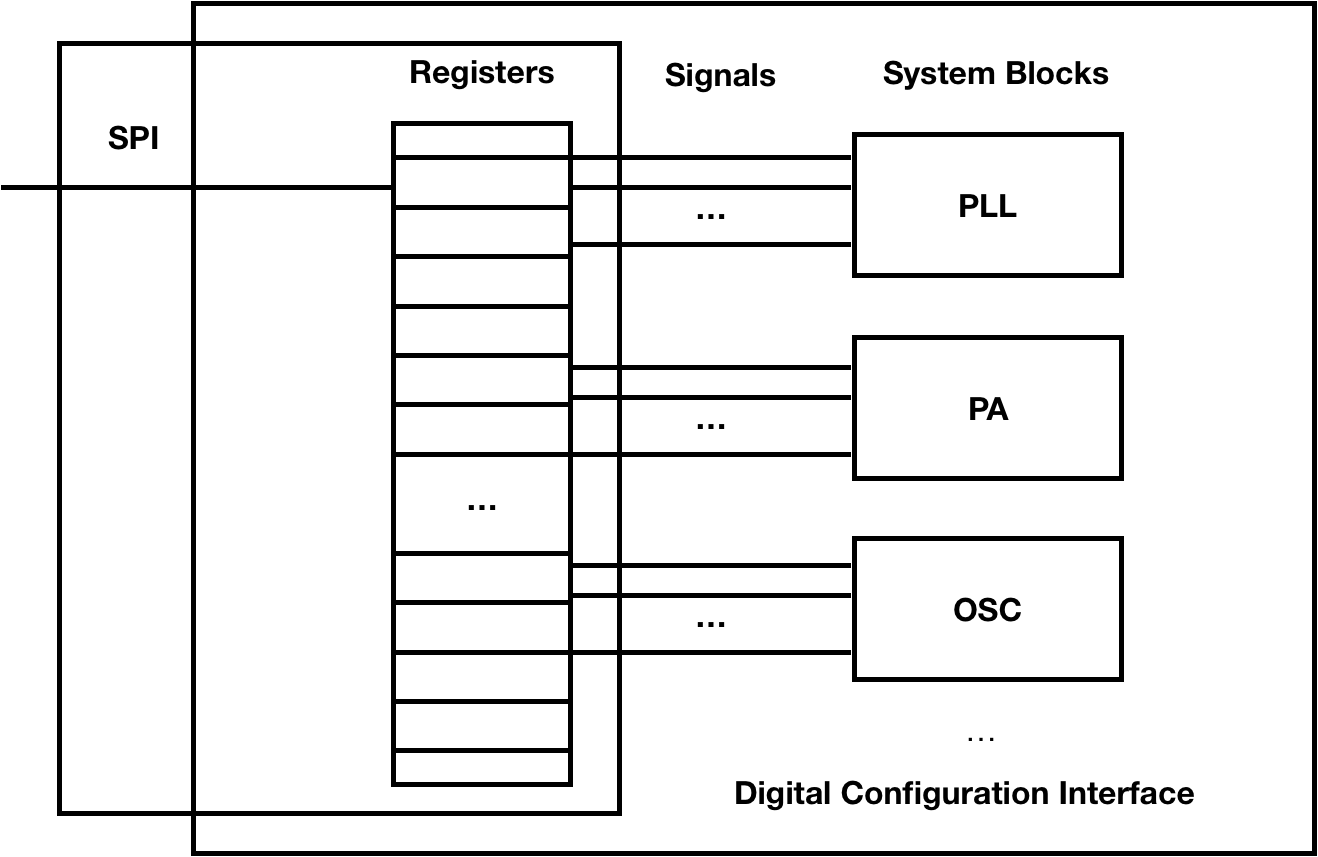
\includegraphics[width = \textwidth]{asic}
\caption{Structure of an ASIC chip\label{fig:Structure of an ASIC Chip}}
\end{figure}

To implement such a digital configuration interface, the designers are required to
\begin{itemize}
\item Define the control and information signals in each system block
\item Define registers and map them to corresponding signals
\item Implement read and write logic for the registers
\item Write documentation of the digital configuration interface
\end{itemize}

The digital configuration interface is implemented in a Hardware Description Language such as VHDL and the documentation is written in LaTeX. Each part of the interface source code and documentation are written by a corresponding system block designer. Finally, there has to be a single designer, let’s say a chip owner, that collects all these VHDL and LaTeX source code and make up a complete SPI interface and documentation.

There are, however, several shortcomings in this manual design approach. First, implementation of the documentation and the VHDL source code can be very tedious and labor intensive. The designers have to write everything completely by hand. However, much of the source code has a strong pattern and can actually be generated by software.

Then, manual implementation of the digital configuration interface can be very error-prone. A good example would be generation of initial values for registers. For each register bit, users have to find out which bit of which signal it is mapped to, and then convert the initial value of the signal from hexadecimal to binary, and get the value of the corresponding signal bit, that is the initial value of this register bit. Some register bits might not be mapped to any signals, then its initial value could be just 0. Finally, concatenate initial value of each register bit and convert it to hexadecimal. The designers have to be very careful not to map a register bit to a wrong signal bit, or write down a wrong value for a register bit.

Also, special attention must be paid to synchronization of the VHDL source code and the LaTeX documentation. For example, when the initial value of a register is updated, the designers have to update the same number everywhere.

Finally, the chip owner has to communicate well with each system block designer. This requires additional efforts, and might cause errors resulted from poor synchronization or communication.

In practice, the chips designed by the Chair can contain decades of system blocks with hundreds of registers, and even more signals. As the complexity of the chips grows, the shortcomings become a serious problem. 

In this background, we propose a software that automates the implementation of the digital configuration interface. The basic idea is simple: the system block designers define the registers and signals and signal-register mappings using the software. They put in documents for each system block, signal or register using a friendly GUI. When the definition is finished, the software can collect all information about the chip, put everything together and generate the VHDL source code and a complete LaTeX documentation automatically.

\begin{figure}[htbp]
\centering
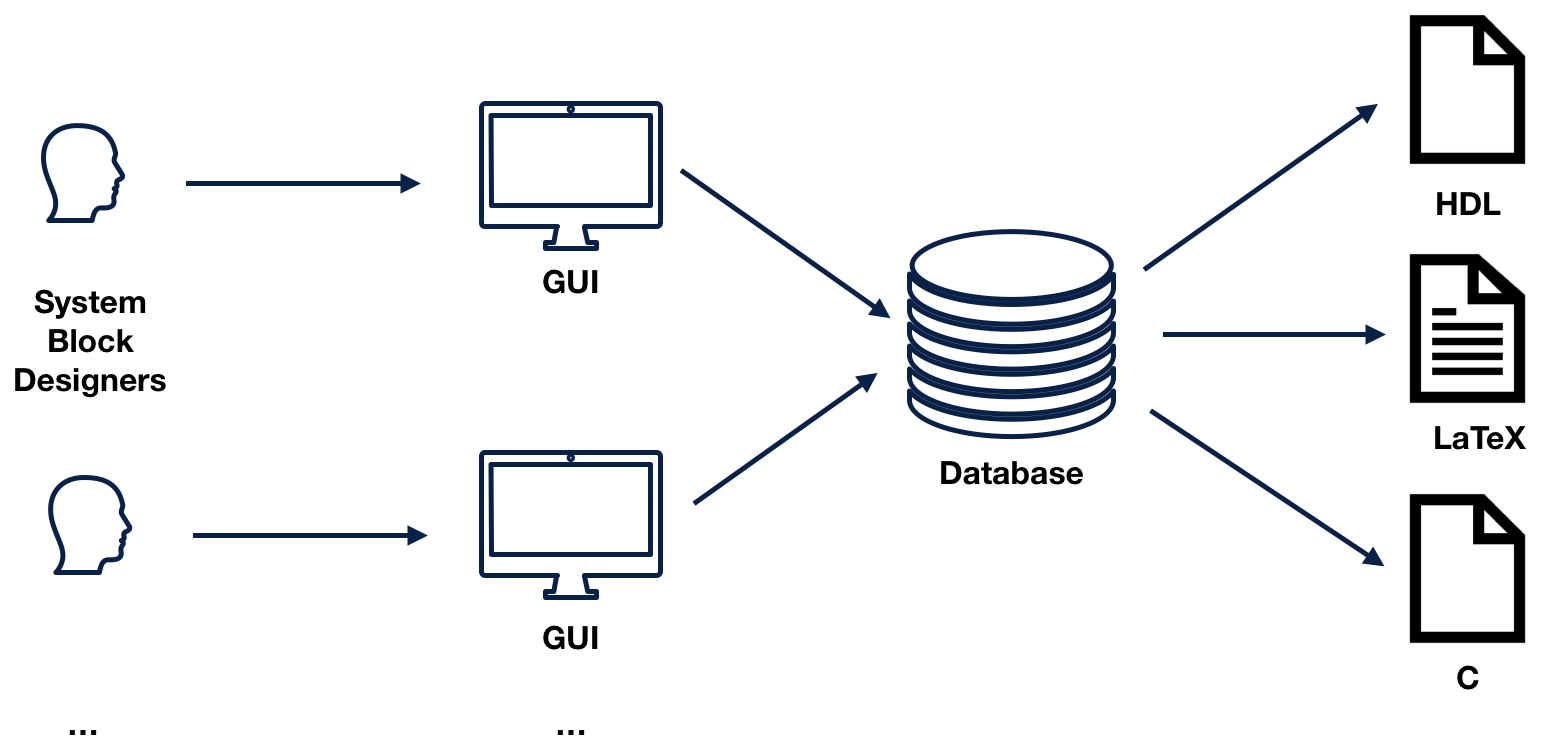
\includegraphics[width = \textwidth]{softwaresolution}
\caption{Proposed Software Solution\label{fig:Proposed Software Solution}}
\end{figure}

Every designer works independently on a single system block, but to generate a complete VHDL source code and documentation, information about all system blocks has to be collected. Due to this fact the software must use a shared data storage which is accessible to all users. We propose to use an open source SQL database system as our data container. With an appropriate database design, we are able to manage the data in a highly secure and efficient way.

The proposed solution has the following great advantages
\begin{itemize}
\item Designers only have to do minimum necessary work, such as defining the name and type of the registers and signals, defining initial values of the signals, mapping signal and register partitions and so on. The rest of work, such as inferring initial values for registers, will be done by the software. By developing a highly friendly user interface, human labor can be reduced to a minimum level. Finally, when definitions of all system blocks are complete, the chip owner do not have to manually collect information. The software shall retrieve all required information from the database and generate the VHDL source code and LaTeX documentation. What the chip owner must do is just some mouse clicks.
\item Synchronization of different outputs is intrinsically ensured. The shared database is the unique data source. Whatever is changed, will be directly reflected on all generations.
\item Errors are less likely to occur, since the most error-prone parts are taken care of by the software. In fact, if all information given by the designers is correct, errors can ideally be eliminated. This requires a highly reliable software, though.
\end{itemize}